% !TEX root = thesis-ex.tex


Hard scatterings in particle collisions result in the production of highly energetic partons that evolve, decay, and eventually form conical sprays of particles called jets. Jet production is well understood in the context of perturbative QCD \cite{PhysRevLett.39.1436}, and can be shown as Figure~\ref{fig:feynman_jet}. It can be described in terms of the parton distribution functions, scattering cross sections, and final state fragmentation functions as shown below:

\begin{figure}[htbp]
\begin{center}
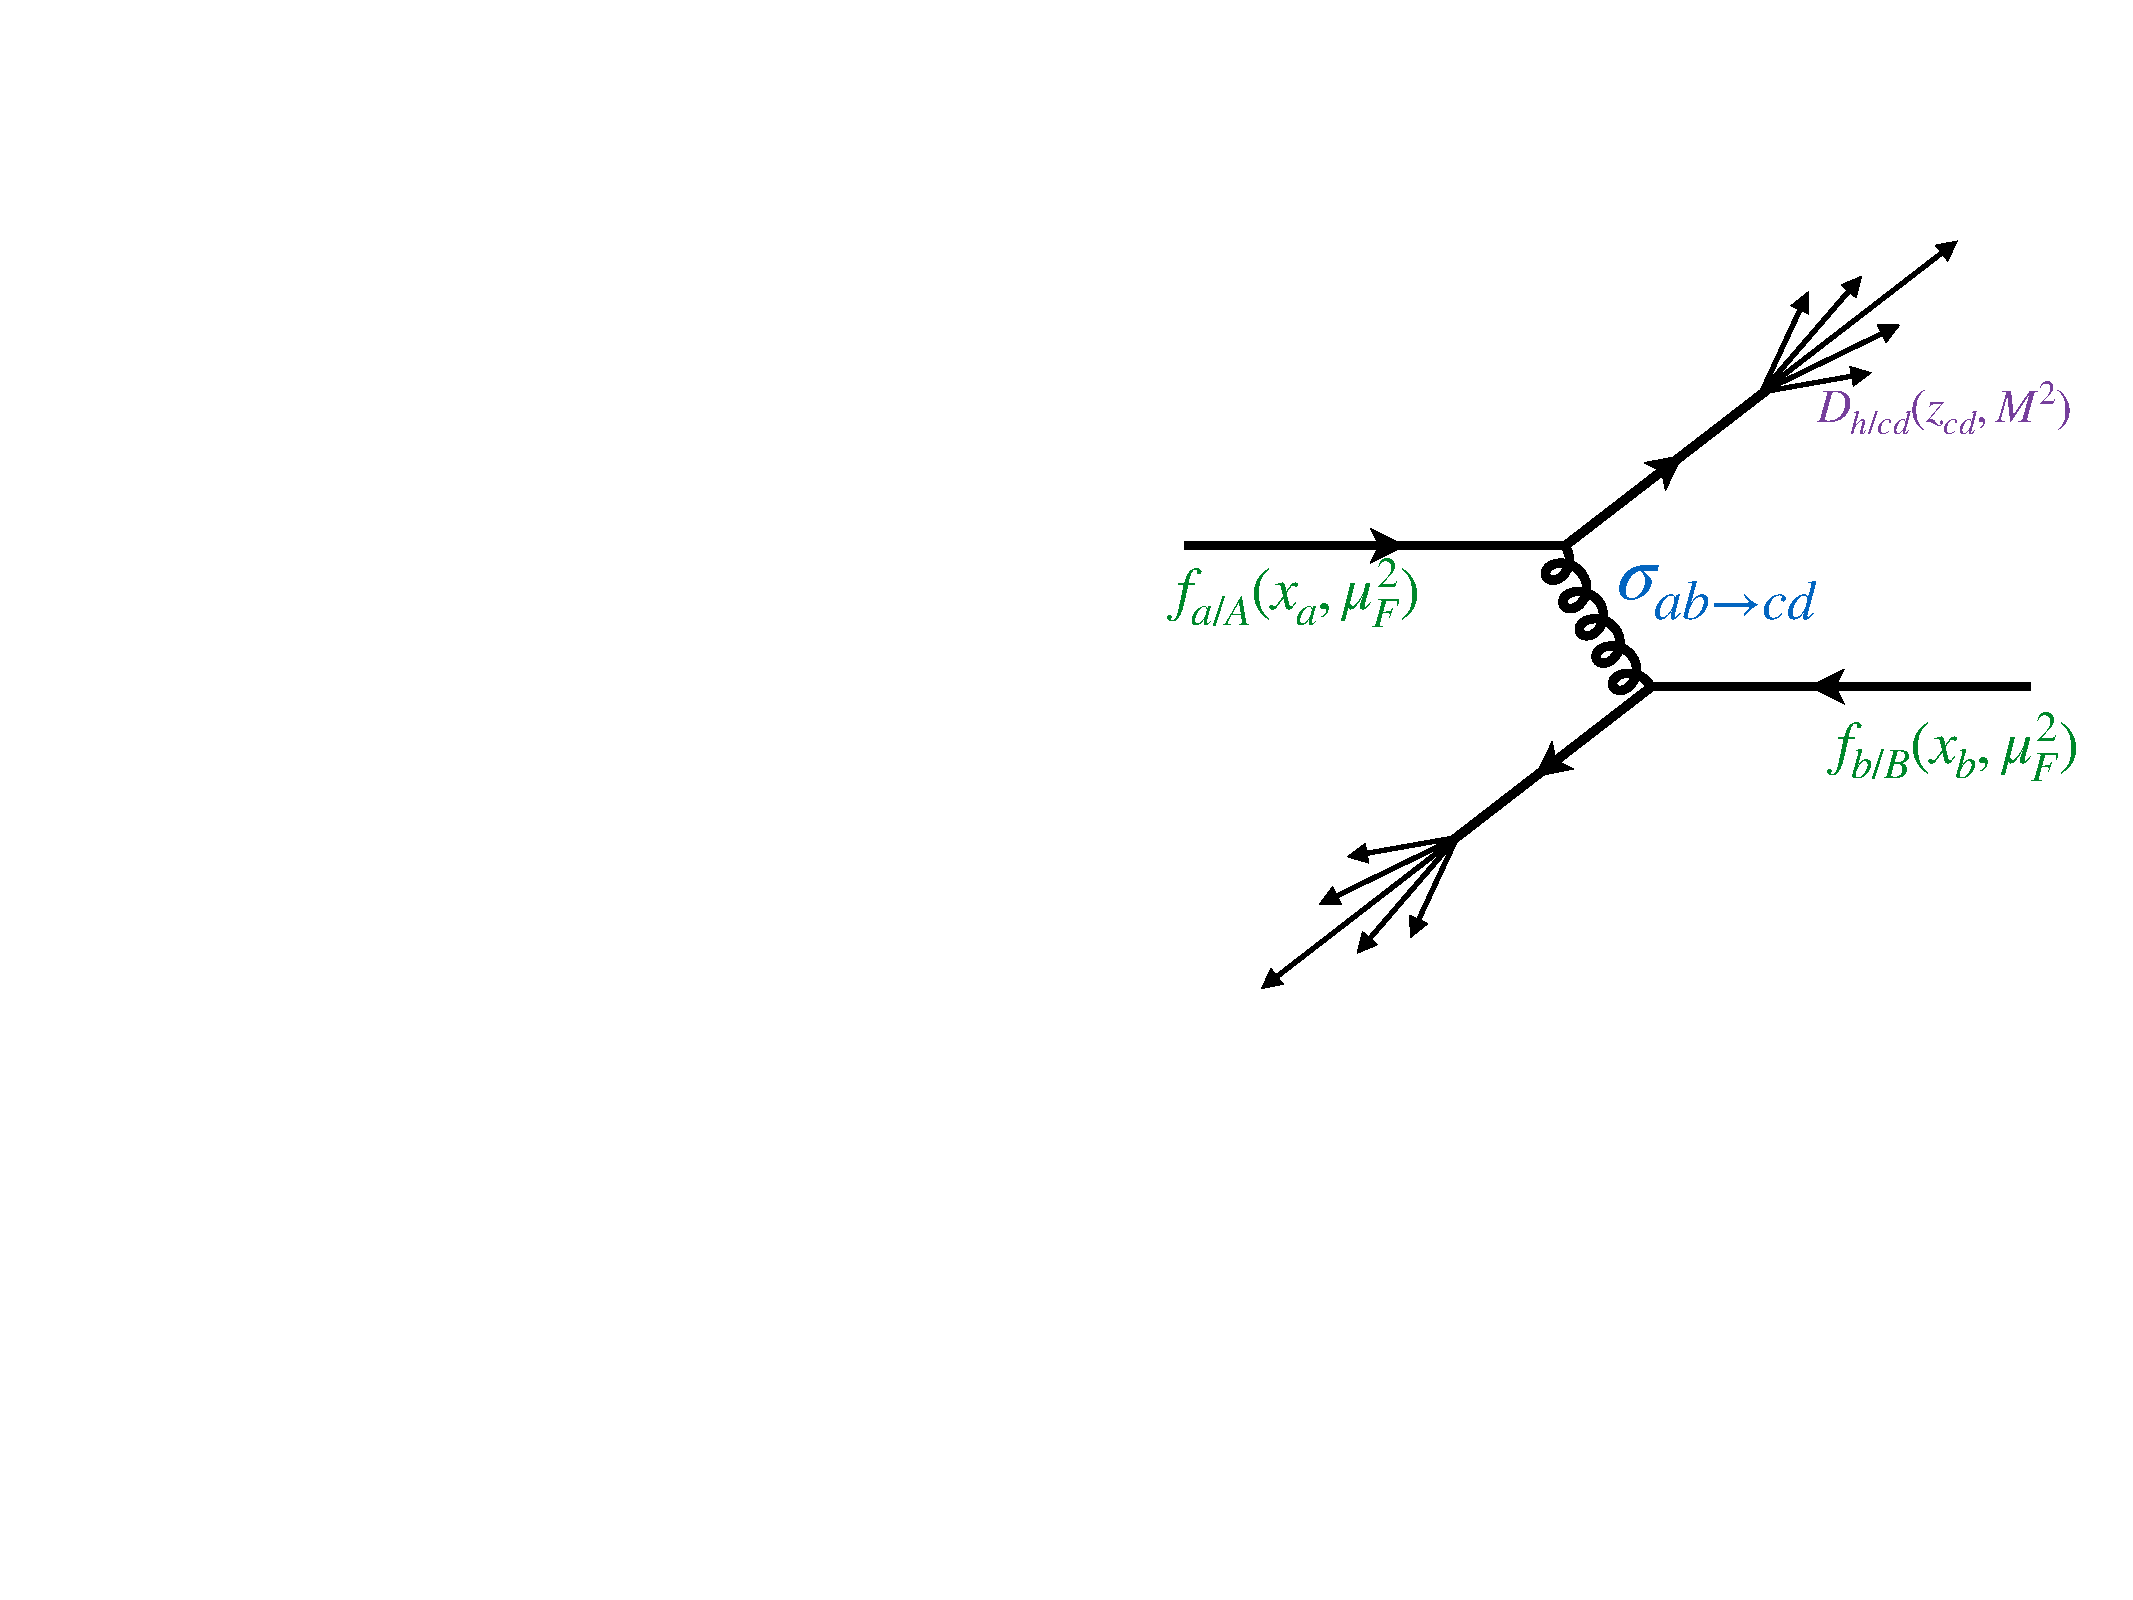
\includegraphics[width=0.55\textwidth]{figures/theory/feynman_jet}
\caption{Jet production from the process $pp \rightarrow hX$, factorizing in terms of the parton distribution functions, scattering cross sections, and jet fragmentation functions. \cite{Qin:2015srf}}
\label{fig:feynman_jet}
\end{center}
\end{figure}

\begin{align}
d \sigma_{pp \rightarrow hX} \approx & \sum_{abjd} \int dx_a \int dx_b \int dz_j f_{a/p} (x_a, \mu_f) \times f_{b/p} (x_b, \mu_f) \\
& \times d\sigma_{ab\rightarrow jd} (\mu_f, \mu_F, \mu_R) \\
& \times D_{j \rightarrow h} (z_j, \mu_f)
\label{eq:jetCS}
\end{align}

where $x_a = p_a/P_A, x_b = p_b / P_b$ are the initial momentum fractions carried by the interacting partons, $z_j = p_h / p_j$ is the momentum fraction carried by the final observed hadron. $f_{a/p} (x_a, \mu_f)$ and $f_{b/p} (x_b, \mu_f)$ are the two parton distribution functions (PDFs), $d\sigma_{ab\rightarrow jd} (\mu_f, \mu_F, \mu_R)$ is the differential cross section for parton scattering and $D_{j\rightarrow }(z_j,\mu_F)$ is the fragmentation function (FFs) for parton $j$ to hadron $h$. $\mu_f$ and $\mu_F$ are the factorization scales and $\mu_R$ is the renormalization scale, and are typically taken to be the same hard scale $Q$. The PDFs characterize the initial state and represent the probability of finding a parton with momentum fraction $x$ (shown in Figure~\ref{fig:bjorkenX}) in the initial hadron, while the FFs describe the probability of fragmenting to a hadron $h$ with given kinematic properties. Both the PDFs and FFs are universal and evolve via the Dokshitzer-Gribov-Lipatov-Altarelli-Parisi (DGLAP) equations \cite{ALTARELLI1977298, Gribov:1972ri, Dokshitzer:1977sg}. 

\begin{figure}[htbp]
\begin{center}
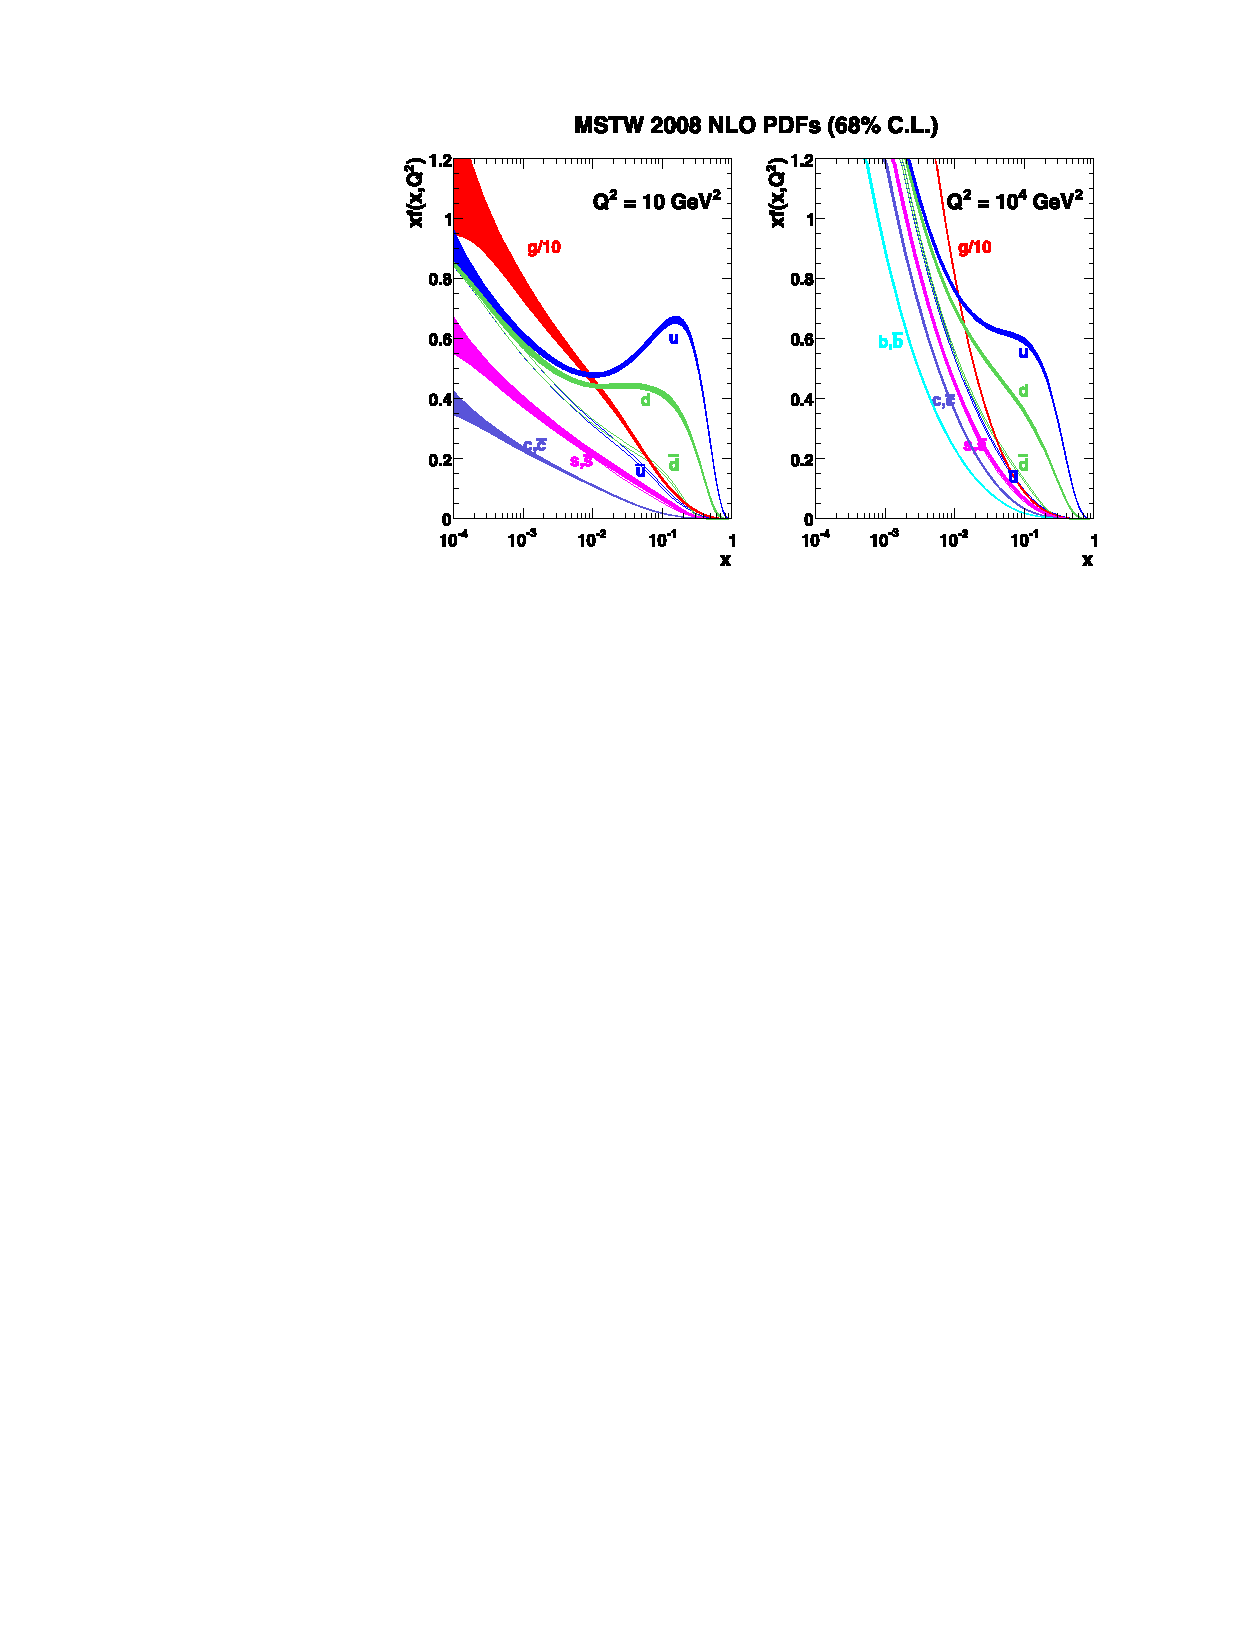
\includegraphics[width=0.55\textwidth]{figures/theory/bjorkenX}
\caption{The next to leading order (NLO) PDFs at (left) $Q^2 = 10 \mathrm{GeV}^2$ and (right) $Q^2 = 10^4 \mathrm{GeV}^2$. The band is the associated one-sigma (68\%) confidence level uncertainty. Taken from \cite{Martin2009}}
\label{fig:bjorkenX}
\end{center}
\end{figure}

Equation~\ref{eq:jetCS} is written at leading order LO and includes contributions from $2\rightarrow2$ cross sections, LO resummed PDFs and FFs, and single loop expression for the strong coupling $\alphas$. At next to leading order (NLO), the contributions from real $2\rigtharrow3$ and virtual $2\rigtharrow2$ processes, as well as the double loop expression for \alphas are included. These calculations describe the inclusive  and  pQCD, NLO calculations hae Next to leading order (NL) calculations that include 
Figure~\ref{fig:incljetCS} shows the inclusive jet cross section as measured by ATLAS in \sqrts = 13 TeV \pp\ collisions. 


\begin{figure}[htbp]
\begin{center}
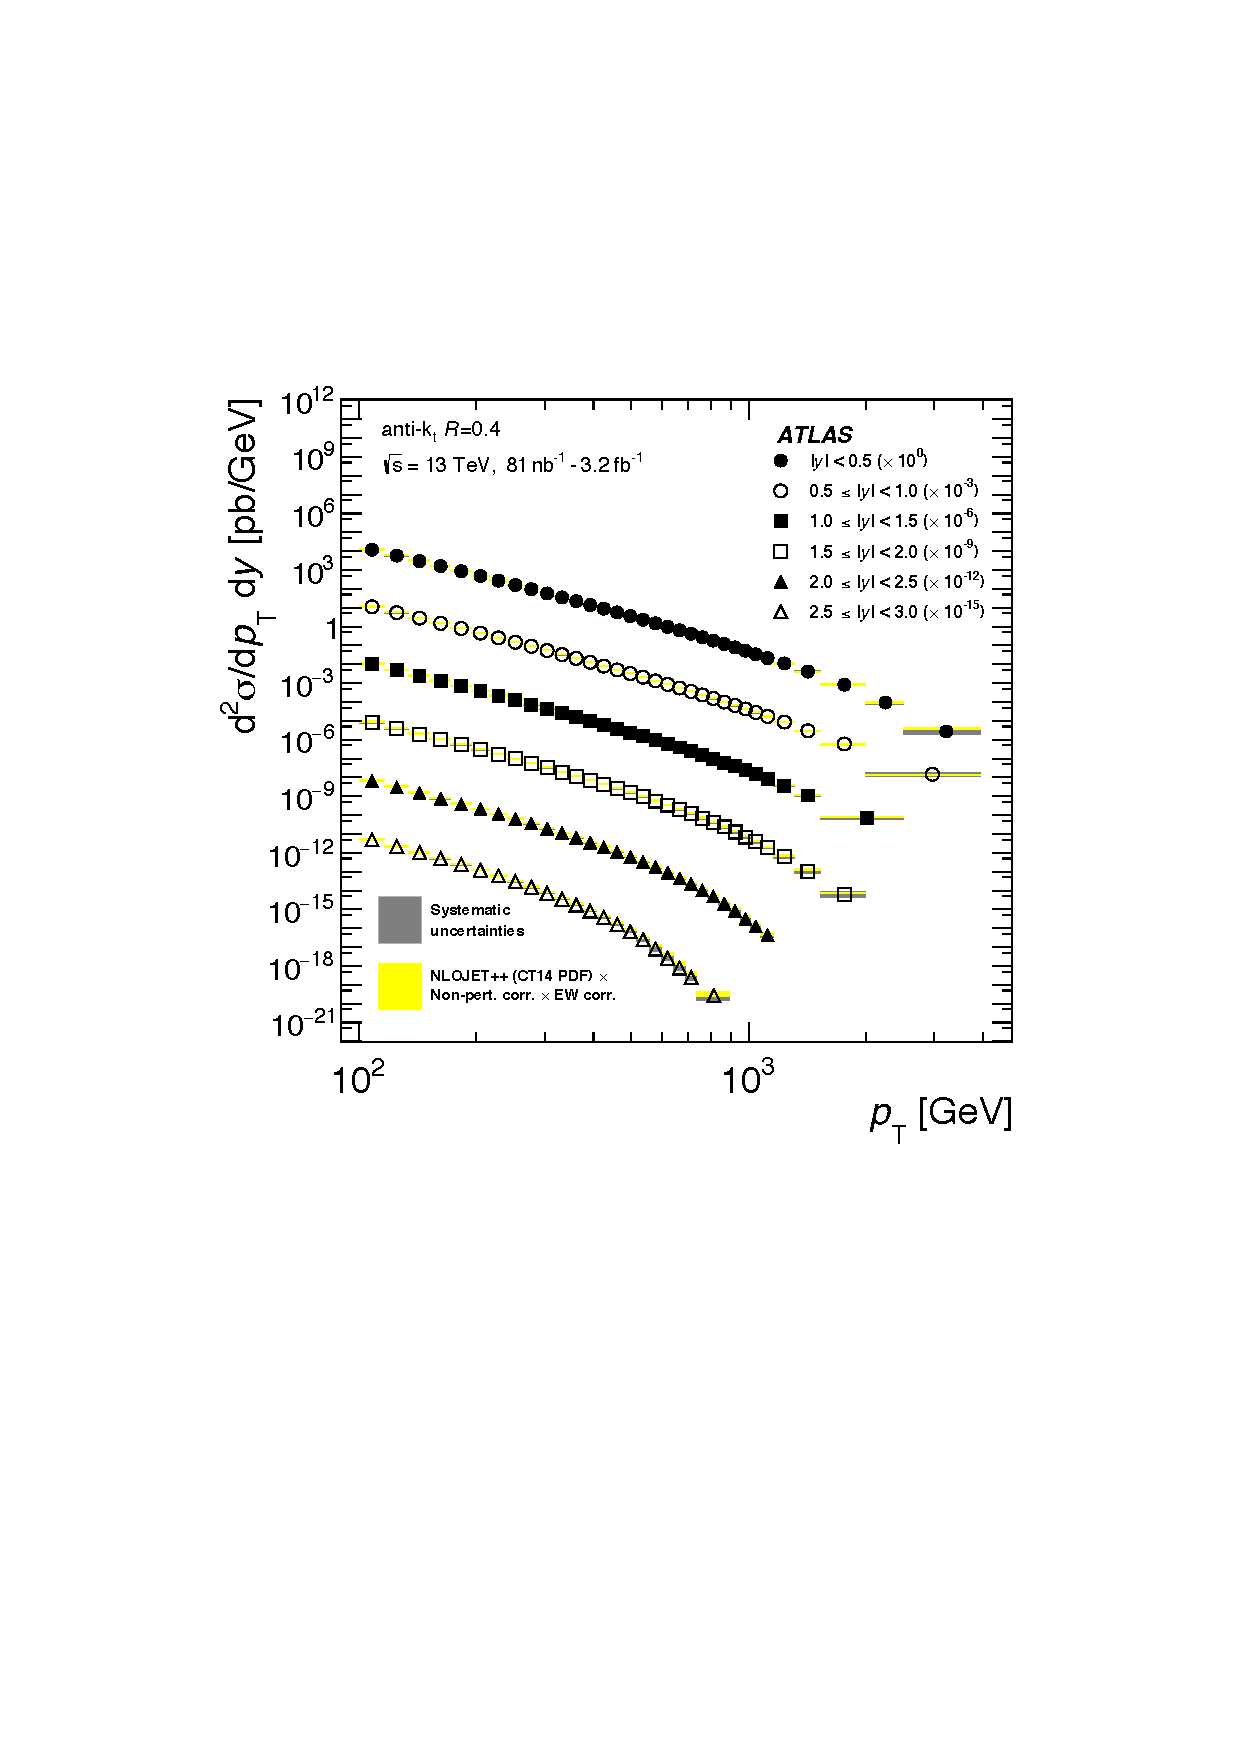
\includegraphics[width=0.55\textwidth]{figures/theory/inclJetCS}
\caption{The inclusive jet cross section as a function of \pt\ and $|y|$ as measured by ATLAS. The data are compared to NLO pQCD calculations. Taken from \cite{Aaboud:2017wsi}}
\label{fig:bjorkenX}
\end{center}
\end{figure}




In heavy ion collisions, jets must traverse the quark gluon plasma. This can result in the jet losing energy and forward momentum \cite{2012176, ATLAS:2017wvp}, while also picking up momentum transverse to the parton direction. Jets can also deposit energy in the medium, creating a wake \cite{Khachatryan2016}. 


In a heavy ion collision where the QGP is formed, the hard scattering interactions between the partons strongly interact with the QGP due to their color charge and are modified and lose energy via collisions with the medium constituents, or gluon bremsstrahlung. 